\documentclass[a4paper,11.5pt]{article}
\usepackage[latin1]{inputenc}
\usepackage[T1]{fontenc}
\usepackage[english]{babel}
\usepackage{graphicx}
\usepackage{amsmath}
\usepackage{amsfonts}
\usepackage{multirow}
\usepackage{booktabs}
\usepackage{bbold}
\usepackage{mathtools}
\usepackage{mathrsfs}
\usepackage{enumitem}
\usepackage{array}
\usepackage{float}

\setlength{\parindent}{0pt}
\DeclarePairedDelimiter{\floor}{\lfloor}{\rfloor}
\DeclarePairedDelimiter{\ceil}{\lceil}{\rceil}

\newcommand{\vt}{\boldsymbol}

\title{Digital Communications - HW4}
\author{Jacopo Pegoraro, Edoardo Vanin}
\date{04/06/2018}

\begin{document}

\maketitle

We want to implement and evaluate the performances of two modulation schemes in the case of uncoded and coded bits. The first system we consider is a matched filter/DFE receiver with single carrier modulation. The information signal in this case is transmitted through the channel and equalized at the receiver by canceling the ISI due to the postcursors of the total impulse response with feedback, while the ISI due to the precursors is reduced by the feedforward filter $c$. In the case of OFDM instead we use a multi-carrier approach and we carry out the equalization by using the \emph{cyclic prefix} method. 

\section*{System setup}

The setup of the system is carried out differently for the uncoded and coded cases. The starting point is a sequence of bits $b_l$ on sampling time $T_{bit}$, produced by a PN sequence with parameter $r=20$ and length $L=2^r-1$ repeated once.

\subsection*{Uncoded}

In the uncoded case the sequence $b_l$ directly mapped into a sequence of QPSK symbols $a_k$ at sampling time $T_a=2T_{bit}$ through a bitmap function that uses Gray coding. At the receiver the detected sequence will pass through an inverse bitmap before the computation of the probability of bit error $P_{bit}$.

\subsection*{Coded}

In the coded case the sequence is first coded using an LDPC encoder with rate $1/2$. This operation produces a sequence of bits $c_m$ with double the length of $b_l$ and sampling time $T_{cod}$. To improve the performances by reducing the effect of burst errors, $c_m$ is passed to an interleaver $43 \times 41$ in which we write the input bits by row and read them by column to perform a scramble.

At this point the resulting bit sequence $c_p'$ at $T_a = 2T_{cod}$ is transmitted using the single carrier and OFDM schemes. At the receiver, once the detection has taken place, the reverse operations are carrier out to derive the detected bit sequence $\hat{b}_l$ and compute $P_{bit}$. In particular a LDPC decoder and a deinterleaver $41\times 43$ are used.

\section*{Single Carrier with DFE}


\section*{OFDM with cyclic prefix}



\begin{figure}[H]
	\begin{center}   
		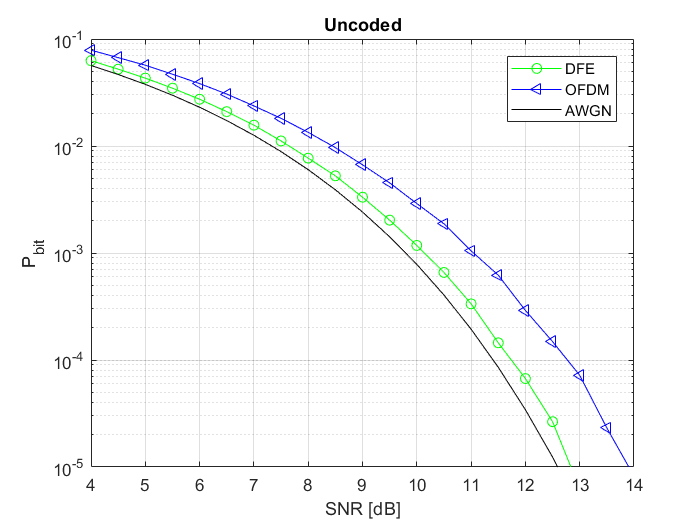
\includegraphics[width=\textwidth]{figs/Pbit_uncoded.png} 
		\caption{$P_{bit}$ obtained for various values of the SNR with DFE equalization and OFDM, no channel coding used.}
		\label{fig:Pbit_uncoded}
	\end{center}
\end{figure}

\begin{figure}[H]
	\begin{center}   
		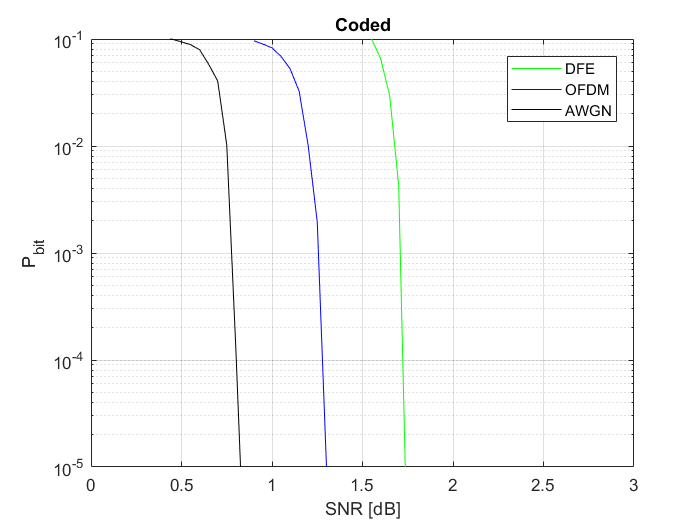
\includegraphics[width=\textwidth]{figs/Pbit_coded.png} 
		\caption{$P_{bit}$ obtained for various values of the SNR with DFE equalization and OFDM, LDPC coding has been used.}
		\label{fig:Pbit_coded}
	\end{center}
\end{figure}
 
\begin{thebibliography}{15}
	
	\bibitem{nevio<3}
	Nevio Benvenuto, Giovanni Cherubini,
	\textit{Algorithms for Communication Systems and their Applications}. 
	Wiley, 2002.
	

	
\end{thebibliography}

\end{document}